\documentclass[12pt]{scrartcl}
\usepackage{graphicx}
\graphicspath{{./}}
\usepackage[sexy]{evan}
\usepackage[normalem]{ulem}
\usepackage{hyperref}
\usepackage{mathtools}
\usepackage{multicol}
\hypersetup{
    colorlinks=true,
    linkcolor=blue,
    filecolor=magenta,      
    urlcolor=cyan,
    pdfpagemode=FullScreen,
    }
\usepackage[most]{tcolorbox}
\renewcommand{\dangle}{\measuredangle}

\renewcommand{\baselinestretch}{1.5}

\addtolength{\oddsidemargin}{-0.4in}
\addtolength{\evensidemargin}{-0.4in}
\addtolength{\textwidth}{0.8in}
% \addtolength{\topmargin}{-0.2in}
% \addtolength{\textheight}{1in} 


\setlength{\parindent}{0pt}

\usepackage{pgfplots}
\pgfplotsset{compat=1.15}
\usepackage{mathrsfs}
\usetikzlibrary{arrows}

\title{Bunch G5-6 WMI Finals}
\author{Azzam Labib (IG: haxuv.world)}
\date{G5-6| \today}
\begin{document}
\maketitle

\section{2020 G6 B}
Certainly, I'll convert all the problems from this competition paper to LaTeX format. Here's the conversion:

\begin{enumerate}
    \item Find the sum of all the 1-digit prime factors of 23464623.

    \item Bind 4 straws which are 2cm in diameter with a $a+b\pi$ cm long string. If both $a$ and $b$ are integers, find $a \times b$. (The knot does not take into consideration.)

    \item Given 4 different positive integers $a$, $b$, $c$, and $d$ that satisfy $\frac{1}{a} + \frac{1}{b} + \frac{1}{c} + \frac{1}{d} = 1$. Find the minimum value of $a+b+c+d$.

    \item Given that the digits of a 4-digit number $A$ are even numbers, the digits of a 4-digit number $B$ are odd numbers, and the digits of a number $C$ are the alternation of odd and even numbers. If $C = A + B$, find the maximum value of $C$.

    \item In Jumping Grid, the player jumps 1 grid or 2 grids forward each time, such as jump from $\square$ to $\square$ or $\square$. If David is at $\square$, how many ways are there for him to jump to $\square$?

    \item If $\angle A = 35^\circ$, $\angle B = 40^\circ$, $\angle C = 30^\circ$, find the degrees of $\angle D + \angle E + \angle F$.

    \item Delete 6 of the 16 figures in the squares so that the numbers of the figures on each row and each column are even numbers. Find the maximum sum of the remaining 10 numbers.

    \item Take 9 numbers from 1--20 without repetition and fill them in a $3 \times 3$ grid so that the sums on each row, each column, and each diagonal are the same. If there are $a$ primes among these 9 numbers at most, and that the largest prime is $b$, find $a \times b$.

    \item The result of $123456789 \times 36 \times 5$ has $a$ 0's, $b$ 1's, and $c$ 2's. Find the 3-digit number $\overline{abc}$.

    \item The picture shows a Sudoku game with number 1 to 5. The number and the math symbol in the top left corner of the frame indicate the result in each frame. For example, "6+" means that the sum of the numbers in the frame is 6. Find the 5-digit number $\overline{ABCDE}$.
\end{enumerate}

% Note: For problems 5, 7, and 10, you may need to include the specific grid or Sudoku diagram as an image or create it using LaTeX drawing commands for a complete representation.

\section{2023 G5 A}
Here's the conversion of all problems in the competition paper to LaTeX:

\begin{enumerate}
    \item The units digit and the tens digit of a 2-digit number are composite numbers that are coprime. When the 2-digit number has the largest value, how many factors does it have?
    
    \item Cut a cuboid whose surface is painted red into several cubes of 1 cm$^3$. Suppose only 3 cubes don't have any red faces, find the volume of the original cuboid in cm$^3$.
    
    \item As shown, ABCD is a square, DE intersects CE at E, DE intersects AC at F, $\angle DEC = 24^\circ$. Find $\angle EFB$.
    
    \item Insert three bamboo poles A, B, and C in the ground at the depth of $x$ cm. If the parts of the three bamboo poles above the ground are $\frac{2}{3}$, $\frac{3}{4}$, and $\frac{1}{3}$ of each of their total lengths, respectively, find the ratio of the lengths of A, B, and C.
    
    \item Below is the math test result of a class of 41 students. Find the median and mode of their scores.
    \begin{tabular}{|c|c|c|c|c|c|c|}
    \hline
    Score & 50 & 60 & 70 & 80 & 90 & 100 \\
    \hline
    Number of People & 1 & 12 & 8 & 13 & 4 & 3 \\
    \hline
    \end{tabular}
    
    \item In a train carriage, $\frac{1}{4}$ of the passengers are young people, $\frac{2}{3}$ of the passengers are middle-aged people, and the rest are elderly people. Suppose there are 6 elderly people, and the number of seats in the carriage is $\frac{3}{4}$ of the number of passengers. How many passengers don't have a seat?
    
    \item The sum of three large, medium, and small numbers is 166. Given that the quotients of the large number divided by the medium number and the medium number divided by the small number are both 3, and their remainders are both 2, find the sum of all the digits of the large number.
    
    \item The number pad "7" on the calculator is broken. If this calculator is used to compute $2023 \times 72$, how many of the following 5 alternatives are correct?
    \begin{itemize}
        \item[A] $2023 \times 80 - 8$
        \item[B] $2023 \times 8 \times 9$
        \item[C] $2023 \times 60 + 12$
        \item[D] $2023 \times (70 + 2)$
        \item[E] $2023 \times 52 + 2023 \times 20$
    \end{itemize}
    
    \item Draw marks on the net and fold it into a solid. Which might be the correct solid? (Include images of the net and the possible solids)
    
    \item In a bag are 11 balls which are marked 1--11. How many balls should Roy take from the bag the least to make sure that at least two of the numbers on the balls are prime numbers?
    
    \item How many 6-digit numbers $x2023y$ are divisible by 286?
    
    \item Find the sum of all the digits of M.
    \[M = (1 - \frac{1}{2}) \times (2 - \frac{2}{3}) \times (3 - \frac{3}{4}) \times \cdots \times (8 - \frac{8}{9}) \times (9 - \frac{9}{10})\]
    
    \item Pour some water in a semicylinder container so that the angle between the rectangular face of the container and the water surface is $45^\circ$. Find the volume of the water in cm$^3$. ($\pi = 3.14$)
    
    \item Draw 3 different diagonals in a regular hexagon at will to make it a line symmetric figure. How many different line symmetric figures can be drawn at most? (If figures look the same after rotation, they are the same one)
    
    \item The last two digits of $1 + 2 + 3 + \cdots + n$ are 03, and its hundreds digit is not 0. If $n$ is no larger than 100, find the sum of all the digits of the smallest $n$.
\end{enumerate}

\section*{2020 WMI Final G06 Paper A}

\subsection*{Problems 1-10. Six points each. Choose the best answer from (A) -- (D).}

\begin{enumerate}
\item $\frac{2}{3} \times 2.4 + 12.4 \times \frac{3}{4} = ?$
\begin{enumerate}[(A)]
    \item 9.9 \item 10.1 \item 10.9 \item 13.9
\end{enumerate}

\item Find the least common multiple of 15, 36, and 90.
\begin{enumerate}[(A)]
    \item 360 \item 270 \item 180 \item 120
\end{enumerate}

\item Determine the next figures of the following pattern.
\begin{figure}[h]
    \centering
    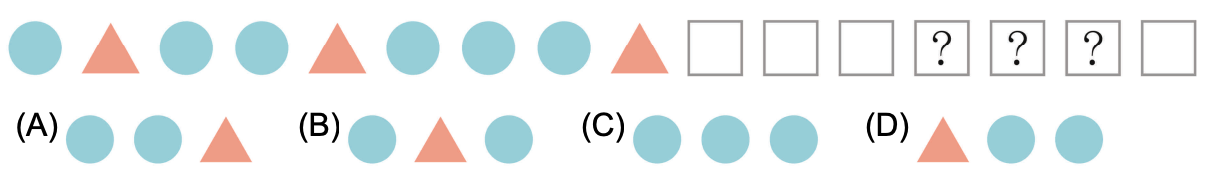
\includegraphics[scale=0.7]{StarGen/0Figure/wmi-2020-6a-num3.png}
\end{figure}

\item If the two figures have the same areas, find the other side length of the figure on the right.
\begin{figure}[h]
    \centering
    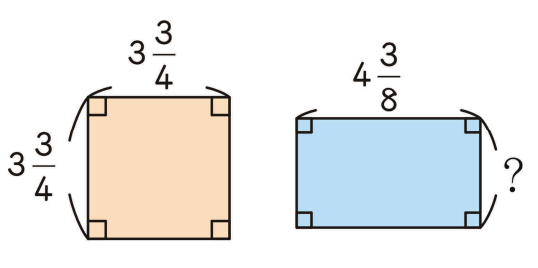
\includegraphics{StarGen/0Figure/wmi-2020-6a-two-rectangle.png}
\end{figure}
\begin{enumerate}[(A)]
    \item $\frac{9}{14}$ \item $3\frac{3}{4}$ \item $2\frac{7}{8}$ \item $3\frac{3}{14}$
\end{enumerate}

\item When Grandpa was 64 years old, Jenny was 4 years old. Now, Grandpa's age is 6 times the age of Jenny's. How old is Jenny now?
\begin{enumerate}[(A)]
    \item 8 \item 10 \item 12 \item 15
\end{enumerate}

\item The record shows the number and type of pitches $x$ that MLB pitcher Johnson threw in a game. What is $y$ approximately?
\begin{center}
    \begin{tabular}{|c|c|c|c|c|}
    \hline
    Fast ball & Slider & Curve & Change-up & Total\\
    \hline
    $48x$ & & $23x$ & & $126x$\\
    \hline
    38\% & 28\% & & y & 100\%\\
    \hline
    \end{tabular}
\end{center}

\begin{enumerate}[(A)]
    \item 18\% \item 16\% \item 22\% \item 20\%
\end{enumerate}

\item There are 27 students in class A. Tom was sick and missed the math test, so the average math score in class A was 69.5. The next day, Tom took the test, and the average math score in class A became 70. What was Tom's math test result?
\begin{enumerate}[(A)]
    \item 83 \item 82 \item 80 \item 78
\end{enumerate}

\item Given a large square on the right. Find $x$ in cm.
\begin{figure}[h]
    \centering
    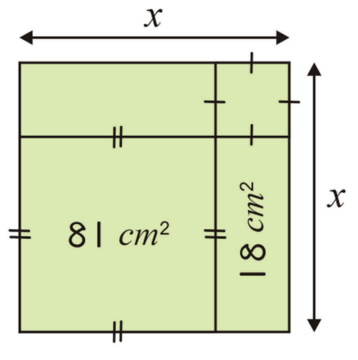
\includegraphics{StarGen/0Figure/wmi-2020-5a-square.png}
\end{figure}
\begin{enumerate}[(A)]
    \item 13 \item 12 \item 11 \item 10
\end{enumerate}

\item At 6:00 a.m., Ben drove from city A to city B at the speed of 90km/hr. After he arrived in city B, he rested for 4 hours, and then he drove back to city A on the same road at the speed of 120km/hr. Given that the distance between the two cities is 358km, when did Ben arrive in city A approximately?
\begin{enumerate}[(A)]
    \item 15:00 \item 16:00 \item 17:00 \item 18:00
\end{enumerate}

\item Find the surface area of the figure on the right in cm$^2$.
\begin{figure}[h]
    \centering
    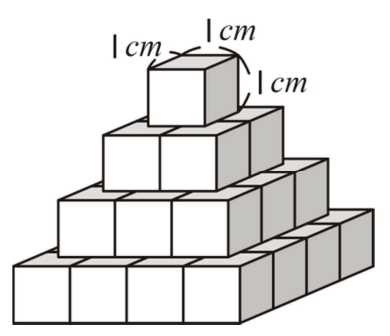
\includegraphics{StarGen/0Figure/wmi-2020-6a-pyramid-of-cubes.png}
\end{figure}
\begin{enumerate}[(A)]
    \item 56 \item 60 \item 72 \item 84
\end{enumerate}
\end{enumerate}

\subsection*{Problems 11-15. Eight points each. Choose the best answer from (A) -- (D).}

\begin{enumerate}[resume]
\item $(1 - \frac{1}{3}) \div (1 - \frac{1}{4}) \div (1 - \frac{1}{5}) \div (1 - \frac{1}{6}) \div (1 - \frac{1}{7}) = ?$
\begin{enumerate}[(A)]
    \item $\frac{4}{7}$ \item $\frac{5}{8}$ \item $\frac{7}{9}$ \item $\frac{14}{9}$
\end{enumerate}

\item The speed of the small boat is 17km/hr, the speed of the large boat is 25km/hr, and the speed of the current is 3km/hr. The two boats start off at the same place, and the large boat starts off 1 hour later than the small boat. If both boats drive downstream, find the distance between the two boats 4 hours after the large boat start off in km.
\begin{enumerate}[(A)]
    \item 18 \item 15 \item 12 \item 9
\end{enumerate}

\item Given that the length and the width of a rectangle are both integers which are larger than 1. Which cannot be the area of the rectangle?
\begin{enumerate}[(A)]
    \item 98 \item 111 \item 135 \item 101
\end{enumerate}

\item Find the volume of the solid. ($\pi = \frac{22}{7}$)
\begin{figure}[h]
    \centering
    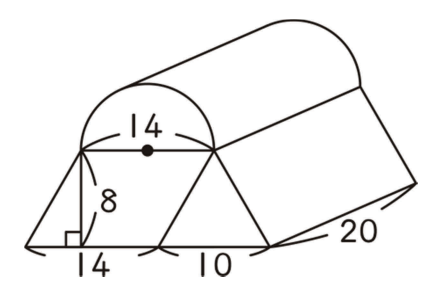
\includegraphics{StarGen/0Figure/wmi-2020-6a-volume-of-solid.png}
\end{figure}
\begin{enumerate}[(A)]
    \item 5000 \item 4840 \item 4580 \item 4060
\end{enumerate}

\item Suppose A and B are numbers from 0--9, and that follow the directions of the arrows will make A become B, find A + B.
\begin{figure}[h]
    \centering
    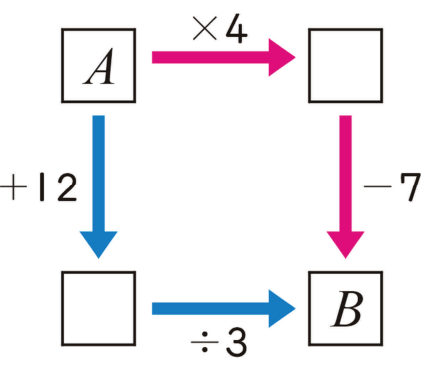
\includegraphics{StarGen/0Figure/wmi-2020-6a-diagram-operation.png}
\end{figure}
\begin{enumerate}[(A)]
    \item 6 \item 7 \item 8 \item 9
\end{enumerate}
\end{enumerate}

\section*{2021 WMI Final G06 Paper B}

\subsection*{Ten points each. Total 100 points.}

\begin{enumerate}
    \item The weights of a bottle of juice, half a bottle of juice, and an empty bottle are shown below, respectively. Find the weight of an empty bottle in $g$.
    
    \begin{figure}[h]
        \centering
        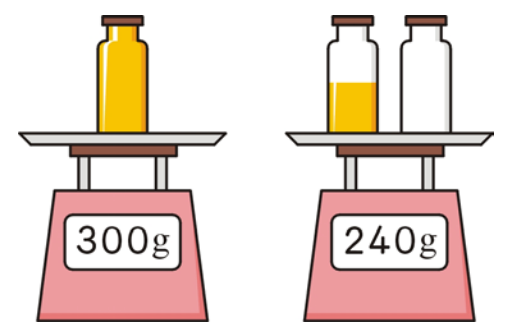
\includegraphics{StarGen/0Figure/wmi-2021-6b-bottle-juice.png}
    \end{figure}
    
    \item Find the smallest prime number $P$ to make $P + 2021$ a perfect square.
    
    \item What is the integer $n$ that makes the sum of $1 + 2 + 3 + \cdots + n$ a 3-digit number which is made up of the same digit?
    
    \item $\dfrac{\dfrac{1}{\frac{1}{10} - \frac{1}{12}}}{\dfrac{1}{\frac{1}{5} - \frac{1}{6}} + \dfrac{1}{\frac{1}{8} - \frac{1}{6}}} = ?$
    
    \item In the picture, the solid is formed by 2 cuboids. Find "?".
    
    \begin{figure}[h]
        \centering
        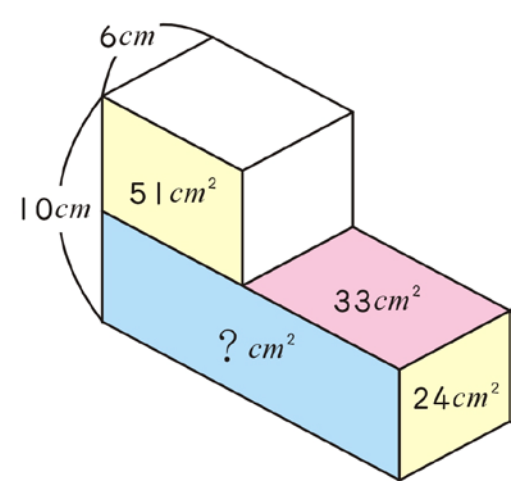
\includegraphics{StarGen/0Figure/wmi-2021-6b-cuboid.png}
    \end{figure}
    
    \item Arrange five positive integers in a row. Start from the second number, each number is not smaller than two times of its previous number. Given that the sum of the five numbers is 2021, find the smallest possible value of the last number in the row.
    
    \item When $1 + 11 + 11^2 + 11^3 + 11^4 + 11^5 + 11^6 + 11^7 + 11^8 + 11^9 + 11^{10}$ is divided by 100, what is the remainder?
    
    \item Below is a circular robot vacuum cleaner. Given that a circular side brush is installed on the edge of it, and the side brush cleans the floor by spinning clockwise around the robot vacuum cleaner. Find the maximum area that the side brush cleans when the robot vacuum cleaner pauses. ($\pi = 3.14$, round to the nearest integer)
    
    \begin{figure}[h]
        \centering
        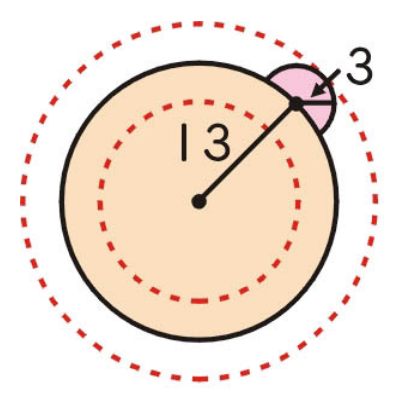
\includegraphics[scale=0.7]{StarGen/0Figure/wmi-2021-6b-robot-vacuum-cleaner.png}
    \end{figure}
    
    \item A rabbit wants to eat the carrot. If the rabbit has to pass all the squares once except the ones with stones, please write down numbers "1234" accordingly to help it get the carrot. Find the sum of the numbers on its way.
    
    \begin{figure}[h]
        \centering
        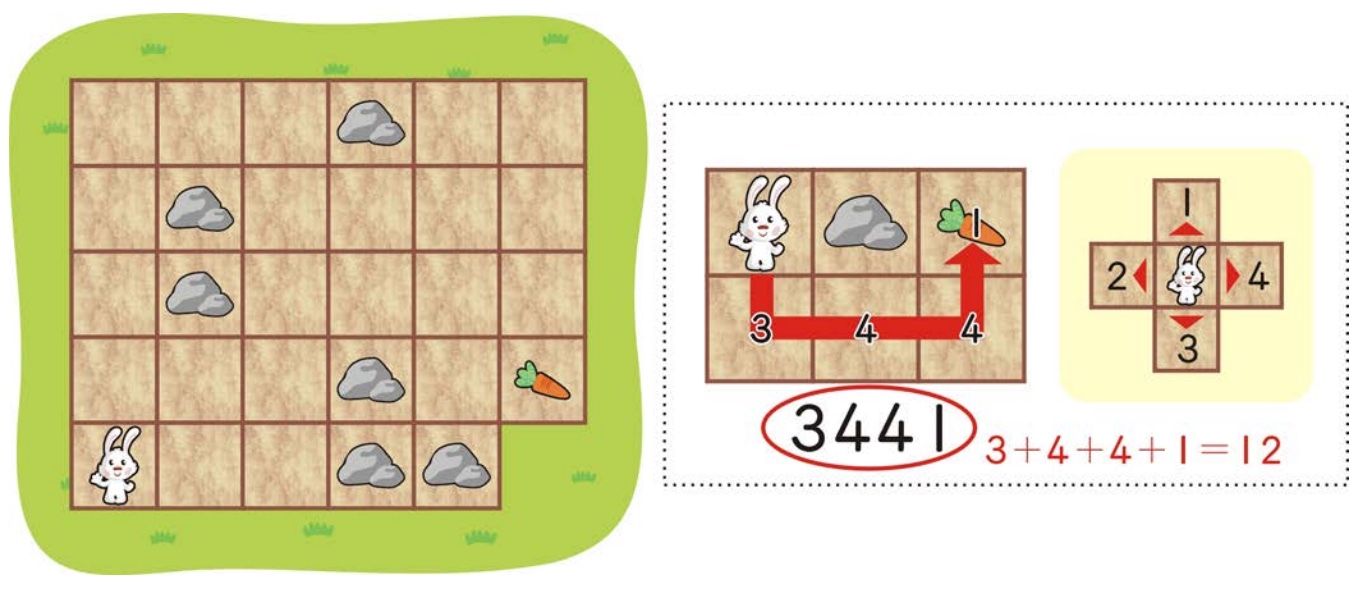
\includegraphics[scale=0.3]{StarGen/0Figure/wmi-2021-6b-rabbit-puzzle.jpeg}
    \end{figure}
    
    \item The picture shows a Sudoku game with numbers 1--5. If the small numbers in the center of the four squares must be the numbers which are written in these four squares, find the 5-digit number $ABCDE$.
    
    \begin{figure}[h]
        \centering
        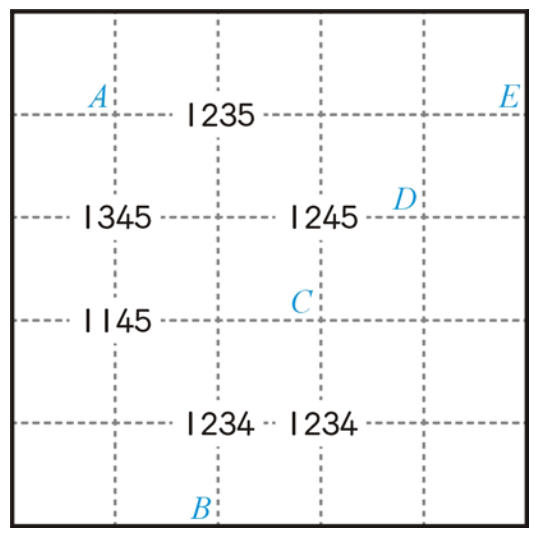
\includegraphics[scale=0.8]{StarGen/0Figure/wmi-2021-6b-sudoku-puzzle.png}
    \end{figure}
\end{enumerate}


\section{2023 G6A}
\subsection*{Problems 1-10. Six points each. Choose the best answer from (A) -- (E).}

\begin{enumerate}
    \item A 5-digit number 215a4 is a multiple of 9. Which number is also a multiple of 9?
    \begin{multicols}{5}
        \begin{enumerate}[(A)]
            \item 3a116
            \item 863a0
            \item 92a39
            \item aa078
            \item 521a73
        \end{enumerate}
    \end{multicols}

    \item Compute $6 \times (1- \frac{1}{2 \times 2}) \times (1- \frac{1}{3 \times 3}) \times (1- \frac{1}{4 \times 4}) \times (1- \frac{1}{5 \times 5}) \times (1- \frac{1}{6 \times 6})$.
    \begin{multicols}{5}
        \begin{enumerate}[(A)]
            \item 3
            \item $3\frac{1}{2}$
            \item 4
            \item $4\frac{1}{2}$
            \item 6
        \end{enumerate}
    \end{multicols}

    \item The figure is the plan view of Terry's house, and each letter represents the length of that side. If $c = 70$ m, $d = 30$ m, $h = 10$ m, find the perimeter of Terry's house in m.
    \begin{figure}[h]
        \centering
        \includegraphics{}
    \end{figure}
    \begin{multicols}{5}
        \begin{enumerate}[(A)]
            \item 210
            \item 220
            \item 230
            \item 240
            \item 250
        \end{enumerate}
    \end{multicols}

    \item Given a fraction whose denominator is larger than its numerator by 4. If 9 is added to both its numerator and the denominator, and the new fraction can be reduced to $\frac{7}{9}$, find the least common multiple of the numerator and denominator of the original fraction.
    \begin{multicols}{5}
        \begin{enumerate}[(A)]
            \item 21
            \item 77
            \item 36
            \item 90
            \item 45
        \end{enumerate}
    \end{multicols}

    \item Mary uses a 36 cm long bamboo stick to weave a cuboid lantern frame whose length, width, and height are different integers in cm. If rice paper should be stuck on the six faces of the lantern, how much rice paper does she need the least in cm$^2$?
    \begin{multicols}{5}
        \begin{enumerate}[(A)]
            \item 52
            \item 46
            \item 40
            \item 36
            \item 34
        \end{enumerate}
    \end{multicols}

    \item What will $x$ be if it is carried to the integral part unconditionally?
    $[(3\frac{2}{7} + x) \div 4\frac{1}{8} - 0.8] \times 11\frac{1}{4} = 6$
    \begin{multicols}{5}
        \begin{enumerate}[(A)]
            \item 3
            \item 1
            \item 4
            \item 2
            \item 5
        \end{enumerate}
    \end{multicols}

    \item Given a cylinder container, the radius of its bottom surface is 8 cm, its height is 10 cm. Put a cylinder whose radius is 4 cm in the container, fill the container with water, and take the cylinder out of the water. What is the height of the water surface now? ($\pi = 3.14$)
    \begin{figure}[h]
        \centering
        \includegraphics{}
    \end{figure}
    \begin{multicols}{5}
        \begin{enumerate}[(A)]
            \item 7 cm
            \item 8.5 cm
            \item 7.5 cm
            \item 8 cm
            \item 6.4 cm
        \end{enumerate}
    \end{multicols}

    \item As shown, a path is on a rectangular land which is $x$ m long and $y$ m wide, and the area besides the path is grassland. Move the left sideline of the path rightward horizontally for $k$ m, and it will overlap with the right sideline of the path. If $x:y = 5:2$, $y:k = 8:1$, find the ratio of the area of the path to the area of the grassland.
    \begin{figure}[h]
        \centering
        \includegraphics{}
    \end{figure}
    \begin{multicols}{5}
        \begin{enumerate}[(A)]
            \item $\frac{1}{19}$
            \item $\frac{1}{16}$
            \item $\frac{1}{15}$
            \item $\frac{1}{20}$
            \item $\frac{2}{19}$
        \end{enumerate}
    \end{multicols}

    \item The average number of five numbers is 30. If one of the numbers is changed to 40, and the new average number becomes 35, find the original number of this changed number.
    \begin{multicols}{5}
        \begin{enumerate}[(A)]
            \item 20
            \item 10
            \item 25
            \item 30
            \item 15
        \end{enumerate}
    \end{multicols}

    \item In a juice shop, it is stipulated that each glass of orange juice should contain $\frac{1}{5}$ measuring cup of real juice. A new clerk John mistook $\frac{1}{5}$ for $\frac{1}{4}$. He didn't find out until he'd made 24 glasses of orange juice, and by then there was only $\frac{1}{3}$ of a full bottle of real juice left. If John made orange juice with the correct proportion from the start, how many glasses of orange juice could be made with a full bottle of real juice?
    \begin{multicols}{5}
        \begin{enumerate}[(A)]
            \item 40
            \item 45
            \item 48
            \item 42
            \item 54
        \end{enumerate}
    \end{multicols}
\end{enumerate}

\subsection*{Problems 11-15. Eight points each. Choose the best answer from (A) -- (E).}

\begin{enumerate}\setcounter{enumi}{10}
    \item In the left figure is a cuboid water container which is 25 cm long, 10 cm wide, and 24 cm high with a partition that is 10 cm long and 1 cm thick inside. Turn on the tap to fill the container with water, and $x$ minutes later the container is full. In the right figure shows the line chart of the water surface height and the water filling time. Find $x$.
    \begin{figure}[h]
        \centering
        \includegraphics{}
    \end{figure}
    \begin{multicols}{5}
        \begin{enumerate}[(A)]
            \item 18.6
            \item 18
            \item 18.2
            \item 18.5
            \item 19
        \end{enumerate}
    \end{multicols}

    \item In a rectangular grid, the length and width of each rectangle are 2 and 1, respectively. Suppose two points A and B are on grid points, point C is also on a grid point, and the area of the triangle whose vertices are points A, B, and C is 1, how many points C satisfy the conditions above?
    \begin{figure}[h]
        \centering
        \includegraphics{}
    \end{figure}
    \begin{multicols}{5}
        \begin{enumerate}[(A)]
            \item 2
            \item 3
            \item 4
            \item 5
            \item 6
        \end{enumerate}
    \end{multicols}

    \item A circular table symbolizes equality. 6 people sit around a circular table whose radius is 60cm at equal distance from each other. Each person sits 20 cm away from the table. When 2 people join them, each of them moves $x$ cm backward and adjusts their seat leftward or rightward so that each part of the arc length among 8 people is the same as each part of the arc length among 6 people originally. Which equation is appropriate?
    \begin{figure}[h]
        \centering
        \includegraphics{}
    \end{figure}
    \begin{multicols}{5}
        \begin{enumerate}[(A)]
            \item $\frac{2\pi(60+20)}{6} = \frac{2\pi(60+20-x)}{8}$
            \item $\frac{2\pi \times 60}{6} = \frac{2\pi(60+x)}{8}$
            \item $2\pi(60+20) \times 6 = 2\pi(60+20+x) \times 8$
            \item $2\pi(60-x) \times 8 = 2\pi(60+x) \times 6$
            \item $\frac{2\pi(60+20)}{6} = \frac{2\pi(60+20+x)}{8}$
        \end{enumerate}
    \end{multicols}

    \item The result of a math test of a class is as follows: The lowest score is 60, the highest score is 100. The score of each student is either a multiple of 2 or 3, and that no two students have the same score. How many students are there in this class at most?
    \begin{multicols}{5}
        \begin{enumerate}[(A)]
            \item 29
            \item 34
            \item 32
            \item 28
            \item 26
        \end{enumerate}
    \end{multicols}

    \item In square ABCD, the area of $\triangle ABE = $ the area of $\triangle BCF = \frac{1}{6}$ of the area of square ABCD. Find the ratio of the area of $\triangle BEF$ to the area of square ABCD.
    \begin{figure}[h]
        \centering
        \includegraphics{}
    \end{figure}
    \begin{multicols}{5}
        \begin{enumerate}[(A)]
            \item $\frac{1}{2}$
            \item $\frac{2}{5}$
            \item $\frac{4}{9}$
            \item $\frac{5}{12}$
            \item $\frac{7}{18}$
        \end{enumerate}
    \end{multicols}
\end{enumerate}


\section{2023 G6B}
\subsection*{Ten points each. Total 100 points.}
\begin{enumerate}
    \item A positive integer $n$ is a perfect square as well as a multiple of 2023. Find the smallest possible value of $n$.

    \item A bag contains balls of three colors: red, yellow, and blue. If the number of blue balls is $\frac{1}{2}$ of the number of yellow balls at most, the number of blue balls is $\frac{1}{3}$ of the number of red balls at least, and the number of yellow balls and blue balls is not exceeding 100, how many red balls are there in the bag at most?

    \item Given a 3-digit number ABC. Add a 6 to its left, and 6ABC is a multiple of 6. Add a 7 to its right, and ABC7 is a multiple of 7. Add an 8 to its left, and 8ABC is a multiple of 8. Add a 9 to its right, and ABC9 is a multiple of 9. Find the value of ABC.

    \item The circumference of circle O is 720 cm. Moving points A and B start off from point P at the same time and move towards different directions along the circumference. Given that point A moves at the speed of 30 cm/sec, point B moves at the speed of 40 cm/sec. If $x$ seconds after the points move, O, A, and B are on a straight line for the first time, and $y$ seconds after the points move, P, A, and B form an isosceles triangle for the second time, find $x + y$.
    \begin{figure}[h]
        \centering
        \includegraphics{}
    \end{figure}

    \item Cut a piece from the cube to make it a heptahedron. If Rachel wants to paint the seven faces with two colors red and blue, how many different ways are there to paint them? (If the solids look the same after rotation or flipping, they are painted in the same way)
    \begin{figure}[h]
        \centering
        \includegraphics{}
    \end{figure}

    \item In the equation below, different letters represent different numbers 0--9. Find ABC + DEF.
    \[ (AB - C) \times (DE - F) \times (G + H + I) \times J = 2023 \]

    \item A square is divided into five rectangles with the same area. Given that one of the rectangles is 4 cm wide, find $x$ in cm.
    \begin{figure}[h]
        \centering
        \includegraphics{}
    \end{figure}

    \item Suppose the units digit of $1^2 + 2^2 + 3^2 + \cdots + 2023^2$ is $x$, and define a new arithmetic operation $a \circ b = \frac{a \times b + 4}{a + 2}$. Find $2023 \circ 2022 \circ 2021 \circ \cdots \circ x \circ (x-1) \circ (x-2)$.

    \item The area of parallelogram ABCD is 100 cm$^2$, and the area of pentagon PQRST is 8 cm$^2$. Find the area of the shaded region in cm$^2$.
    \begin{figure}[h]
        \centering
        \includegraphics{}
    \end{figure}

    \item Fill 1--25 in a $5 \times 5$ grid without repetition to make the sum of the numbers in each row, column, and diagonal in the $5 \times 5$ grid and the colored $3 \times 3$ grid the same. Find the multi-digit number ABCD. (Ex: A = 15, B = 3, C = 22, D = 1, ABCD $\rightarrow$ 153221)
    \begin{figure}[h]
        \centering
        \includegraphics{}
    \end{figure}
\end{enumerate}

\section*{2020 WMI Final G05 Paper A}

\subsection*{Problems 1-10. Six points each. Choose the best answer from (A) -- (D).}

\begin{enumerate}
\item $9 \times 0.1 + 17 \times 0.02 = ?$
\begin{enumerate}[(A)]
    \item 1.04 \item 1.07 \item 1.24 \item 1.34
\end{enumerate}

\item Which number below has the most factors?
\begin{enumerate}[(A)]
    \item 169 \item 98 \item 90 \item 62
\end{enumerate}

\item $60500\text{cc} = ( )\text{ l }( )\text{ml}$
\begin{enumerate}[(A)]
    \item 60 l 500 ml \item 6 l 5000 ml \item 6 l 500 ml \item 6 l 50 ml
\end{enumerate}

\item Unfold the solids below. Which has the most rectangles?
% Note: The actual images would need to be included here

\item $(125 \times 6) \div 5 + (75 \times 5) \div 3 = ?$
\begin{enumerate}[(A)]
    \item 200 \item 245 \item 275 \item 295
\end{enumerate}

\item $57.132 = ?$
\begin{enumerate}[(A)]
    \item $5 \times 10 + 7 \times 1 + 2 \times \frac{1}{1000} + 3 \times \frac{1}{100} + 1 \times \frac{1}{10}$
    \item $5 \times 10 + 7 \times 1 + 1 \times \frac{1}{1000} + 3 \times \frac{1}{100} + 2 \times \frac{1}{10}$
    \item $5 \times 10 + 7 \times 1 + 3 \times \frac{1}{1000} + 2 \times \frac{1}{100} + 1 \times \frac{1}{10}$
    \item $5 \times 10 + 3 \times 1 + 2 \times \frac{1}{1000} + 3 \times \frac{1}{100} + 1 \times \frac{1}{10}$
\end{enumerate}

\item Find the shaded area of the figure in cm$^2$.
% Note: The actual figure would need to be included here
\begin{enumerate}[(A)]
    \item 288 \item 280 \item 272 \item 256
\end{enumerate}

\item Harden is a famous shooter in the NBA, and his three-point field goal percentage is $x\%$ in 2020. If he makes 843 three-pointers this year, how many of them score?
\begin{enumerate}[(A)]
    \item $843x$ \item $8.43x$ \item $3x$ \item $0.3x$
\end{enumerate}

\item $\frac{4}{5} : \frac{3}{4} = 32 : \square$, $\square = ?$
\begin{enumerate}[(A)]
    \item 24 \item 28 \item 30 \item 40
\end{enumerate}

\item The volume of a cuboid is 108cm$^3$. If its length and width are 8cm and $2\frac{1}{4}$cm, respectively, find its height in cm.
\begin{enumerate}[(A)]
    \item 6 \item 7 \item 8 \item 9
\end{enumerate}
\end{enumerate}

\subsection*{Problems 11-15. Eight points each. Choose the best answer from (A) -- (D).}

\begin{enumerate}[resume]
\item Ann computes $36 + 14 \times (8 - 5)$. Is the process "correct" (✓)? Or, does a "mistake" (×) occur at a certain step?
\begin{enumerate}[(A)]
    \item ✓ \item ×, step 1 \item ×, step 2 \item ×, step 3
\end{enumerate}

\item Find the surface area of the solid in cm$^2$.
% Note: The actual figure would need to be included here
\begin{enumerate}[(A)]
    \item 36 \item 42 \item 45 \item 54
\end{enumerate}

\item Among fractions whose denominators are 18, how many of them are larger than $\frac{1}{6}$ yet smaller than $\frac{4}{9}$?
\begin{enumerate}[(A)]
    \item 8 \item 6 \item 5 \item 4
\end{enumerate}

\item Given a large square on the right. Find $x$ in cm.
% Note: The actual figure would need to be included here
\begin{enumerate}[(A)]
    \item 13 \item 12 \item 11 \item 10
\end{enumerate}

\item How many numbers satisfy the three conditions below?
\begin{itemize}
    \item[(i)] A 3-digit number which is larger than 700.
    \item[(ii)] A multiple of 11.
    \item[(iii)] Not a multiple of 2.
\end{itemize}
\begin{enumerate}[(A)]
    \item 24 \item 15 \item 13 \item 12
\end{enumerate}
\end{enumerate}

\section*{2020 WMI Final G05 Paper B}

\subsection*{Ten points each. Total 100 points.}

\begin{enumerate}
\item $2-(2+4)+(2+4+6)-(2+4+6+8)+\cdots-(2+4+\cdots+96)+(2+4+\cdots+98)=?$

\item If both $n-1$ and $n+1$ are primes, the positive integer $n$ is called a "prime interlude". Find the number of "prime interludes" among 2-digit numbers.

\item Write figures 1, 2, 3, 4, 5, 6, 7, 8, and 9 into the squares in a different order to make the sum of each set of upper figure and lower figure a perfect square. How do these 9 figures arranged from left to right?
% Note: The actual diagram would need to be included here

\item Suppose $A \bowtie B = A \times B + A + B$. Find $(20 \bowtie 20) \bowtie (20 \bowtie 20)$.

\item The figure is formed by a regular hexagon, 6 squares, and 6 small regular triangles. Given that the area of $\triangle ABC$ is 12cm$^2$, find the sum of the areas of the 6 shaded small regular triangles in cm$^2$.
% Note: The actual figure would need to be included here

\item Delete 6 of the 16 figures in the squares so that the numbers of the figures on each row and each column are even numbers. Find the maximum sum of the remaining 10 numbers.
% Note: The actual figure would need to be included here

\item Fill up a container with water. Put iron ball A in the container and take it out. Then, put iron ball B in the container and take it out. In the end, put iron ball C in the container. Given that the amount of spilling water at the second time is $\frac{1}{3}$ of the amount of spilling water at the first time, and the amount of spilling water at the third time is twice the amount of spilling water at the first time. If the volume of iron ball A is 30cm$^3$, find the volume of iron ball C in cm$^3$.

\item Take 9 numbers from 1--20 without repetition and fill them in a $3 \times 3$ grid so that the sums on each row, each column, and each diagonal are the same. If there are $a$ primes among these 9 numbers at most, and that the largest prime is $b$, find $a \times b$.

\item Given 4 different positive integers $a$, $b$, $c$, and $d$ that satisfy $\frac{1}{a} + \frac{1}{b} + \frac{1}{c} + \frac{1}{d} = 1$. Find the minimum value of $a+b+c+d$.

\item The picture shows a Sudoku game with number 1 to 5. The number and the math symbol in the top left corner of the frame indicate the result in each frame. For example, "6+" means that the sum of the numbers in the frame is 6. Find the 5-digit number $\overline{ABCDE}$.
% Note: The actual Sudoku grid would need to be included here

\end{enumerate}


\end{document}